\scanpage{54}
\textcircled{\scriptsize 13} L'ens des $18$ triades de $S$ contenues dans un des $X_\alpha$ est en corr. biunivoque avec \deleted{l'ens} le sous-ens $T$ de $I\times A$ formé des couples $(i,\alpha)$ avec $p(i)\ne\alpha$, en associant à un tel couple la triade \inserted{$\tau_{i,\alpha}\subset X_\alpha$} formée des $A\in S\subset\mathcal P_2(I)$ tels que $p(A)=\Lambda-\{\alpha\}$, $A\ni i$. \deleted{\unsure{dira|distincts} $\unsure{\tau_{i,\alpha}\subset}$} La triade opposée à $\tau_{i\alpha}$ est $\tau_{i,\deleted{\unsure{\beta}}\beta'}$, où \deleted{\unsure{$\beta$ est l'él.}} \inserted{$\beta'$} \inserted{l'autre} él. de \deleted{\unsure{$A$|$\Lambda$}} $A-\{p(i)\}$. Les deux triades \deleted{\unsure{bi}}liées à $\tau_{i,\alpha}$ sont $\tau_{j,\unsure{\beta'|\beta}},\tau_{k,\unsure{\beta'|\beta}}$, où $j,k$ sont les \inserted{2 autres} élémts de \deleted{$p^{-1}(p(i))$} $I$ au dessus de $p(i)$. Les deux triades \uline{biliées} à $\tau_{i,\alpha}$ sont $\tau_{j,\beta}\deleted{\unsure{\alpha}},\tau_{k,\beta}$. L'hexagone formé de ces six triades est formé de l'ens des $\tau_{i,\alpha}$ tels que $p(i)=r$ soit donné. L'ens de ces hex. est donc en corr. $1$-$1$ avec $A$ [$:$ l'hexagone $H$ correspondent le complémentaire de sa réunion dans $S$]

\figure{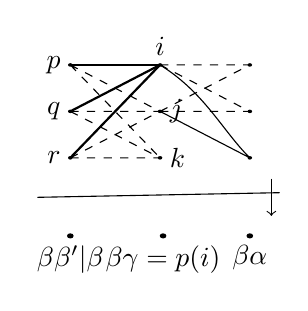
\begin{tikzpicture}[x=.76cm,y=.59cm]
\foreach \x in {0,1.5,3}{\foreach \y in {0,1,2}{\fill (\x,\y) circle (.038);}}
\foreach \y in {0,1,2}{\draw[thick] (0,\y)--(1.5,2);}
\draw[dashed] (0,2)--(1.5,1) (0,2)--(1.5,0) (0,1)--(1.5,1) (0,1)--(1.5,0) (0,0)--(1.5,0) (0,0)--(1.5,1);
\draw[dashed] (1.5,2)--(3,2) (1.5,2)--(3,1) (1.5,1)--(3,1) (1.5,1)--(3,2);
\draw (1.5,2) .. controls (2.25,1.4) and (2.55,.57) .. (3,0) (1.5,1)--(3,0);
\node[left] at (0,2) {$p$};\node[left] at (0,1) {$q$};\node[left] at (0,0) {$r$};
\node[above] at (1.5,2) {$i$};\node[right] at (1.5,1) {$j$};\node[right] at (1.5,0) {$k$};
\draw (-.55,-.85)--(3.5,-.75);\draw[->] (3.36,-.45)--(3.36,-1.25);
\foreach \x in {0,1.55,3}{\fill (\x,-1.68) circle (.056);}
\node[below] at (0,-1.68) {$\deleted{\unsure{\beta}}\unsure{\beta'|\beta}$};
\node[below] at (1.55,-1.68) {$\deleted{\unsure{\beta}}\unsure{\gamma}=p(i)$};
\node[below] at (3,-1.68) {$\deleted{\unsure{\beta}}\alpha$};
\end{tikzpicture}}

\deleted{\textcircled{\scriptsize 14} L'ens \inserted{à $6$ él.} des couples formés d'un des \deleted{\unsure{2}} bitriangles $X_\alpha$, et d'une \uline{coorientation} de $X_\alpha$, est $\simeq$ l'ens des \deleted{\unsure{couples}} couples $(\alpha,\beta)\in A^2$ \deleted{\unsure{ou}} avec $\beta\ne\alpha$ (i.e. à l'ens des repères $(\alpha,\beta,\gamma)$ de l'ens $A$ de cardinal $3$), à $(\alpha,\beta)$ correspond le}
% archive sheet number: 53
